\section{Direct Dynamics}
Previously, we studied \emph{kinematics}, which describes the motion of a robot without considering the forces that cause it. We now turn to \emph{dynamics}, which studies the forces that cause the motion. The \emph{direct dynamics} problem consists in finding the motion of a robot given the forces applied to it.

\subsection{Physical equations}
The motion of a robot is governed by the laws of physics. The \emph{Newton-Euler} equations describe the motion of a rigid body in space. They are a set of differential equations that relate the forces and torques applied to the body to its translational and rotational motion. The equations are given by:
\begin{equation}
    \tag{Newton's equation}
    m_k\underline{\ddot{x}}_k = f_k
\end{equation}
for the translational motion, and:
\begin{equation}
    \tag{Euler's equation}
    I_k\underline{\dot{\omega}}_k + \underline{\omega}_k\times I_k\underline{\omega}_k = \tau_k
\end{equation}
for the rotational motion. Here, $m_k$ is the mass of the body, $f_k$ is the force applied to it, $I_k$ is the inertia matrix, $\underline{\omega}_k$ is the angular velocity, and $\tau_k$ is the torque applied to the body. The equations are written in the body frame of the body $k$, whose origin coincides with the body's center of mass.

Almost all physical problems, from mechanics to relativity, follow the \emph{least-action principle}. This principle states that the actual motion of a system is the one that minimizes a certain quantity, called the \emph{action}. In mechanics, it corresponds to the minimization of the integral of the kinetic-potential energies over time.

We can define $\Ds$ to be a kinetic metric of least deviation between the actual motion of the robot and the desired motion:
\begin{equation}
    \Ds := \sum_{k=1}^n \frac{1}{2}(\ddot{x}_k - \underline{\ddot{x}}_k)^\tp m_k (\ddot{x}_k - \underline{\ddot{x}}_k) + \frac{1}{2}(\dot{\omega}_k - \underline{\dot{\omega}}_k)^\tp I_k (\dot{\omega}_k - \underline{\dot{\omega}}_k)
\end{equation}
Formally, the least-action principle states that the actual motion of the robot is the one that minimizes $\Ds$. We can find the actual motion by solving the following optimization problem:
\begin{equation}
    \min_{\ddot{x}_k, \dot{\omega}_k} \Ds
\end{equation}

In the joint space, we can write the equations of motion as:
\begin{equation}
    M(q)\ddot{q} + C(q, \dot{q}) - F(q) = 0
\end{equation}
where $M(q)$ is the mass matrix, $C(q, \dot{q})$ is the Coriolis matrix, and $F(q)$ is the vector of forces applied to the joints.

\subsection{Contact forces}
The poly-articulated system dynamics is driven by the Lagrangian dynamics. If we consider the contact forces, we can write the equations of motion as:
\begin{equation*}
    \underbrace{M(q)}_{\text{Mass matrix}}\ddot{q} + \underbrace{C(q, \dot{q})}_{\text{Coriolis}} + \underbrace{G(q)}_{\text{Gravity}} = \underbrace{\tau}_{\text{Motor torque}} + \underbrace{J_c^\tp(q)\lambda_c}_{\text{External forces}}
\end{equation*}

With this equation in mind, the direct dynamics problem consists in finding the motion of the robot given the forces applied to it. Schematically, the problem can be written as:
\begin{equation*}
    \ddot{q} = \text{ForwardDynamics}(q, \dot{q}, \tau, \lambda_c)
\end{equation*}
This is used in simulation, and can be solved using the articulated body algorithm.

Conversely, the \emph{inverse dynamics} problem consists in finding the forces applied to the robot given its motion. Schematically, the problem can be written as:
\begin{equation*}
    \tau = \text{InverseDynamics}(q, \dot{q}, \ddot{q}, \lambda_c)
\end{equation*}
This is used in control, and can also be solved by integrating the equations of motion over time (recursive Newton-Euler algorithm).

Note that naive algorithms for solving the direct dynamics problem have a complexity of $O(n^3)$, which is prohibitive for large systems. However, the articulated body algorithm has a complexity of $O(n)$, which makes it tractable for large systems. Such improvements come from the structure of the mass matrix, which is often sparse since parts of the robots are not connected. Similarly, the Jacobian of the contact forces is often sparse, which can also be exploited to reduce the complexity of the problem.

An important aspect of the direct dynamics problem is the computation of $\lambda_c$. Multiple approaches, corresponding to different contact models, can be used:
\begin{itemize}
    \item Soft contact: using a spring-damper model
    \item Rigid contact: using a bilateral or unilateral contact model
    \item Mixed contact: using a relaxed contact model
\end{itemize}
we will study these models in more detail in the next sections.

\subsection{Soft contact}
The soft contact model is used when the contact between the robot and the environment is soft, i.e. when the robot can penetrate the environment. This is one of the simplest contact model, which is both very intuitive and straightforward to implement. 

The model is based on a spring-damper system, where the contact force is proportional to the penetration depth and the relative velocity between the robot and the environment. The spring will push the robot away from the environment (proportionally to the penetration $p$), while the damper will slow down the relative motion between the robot and the environment (proportionally to the speed $\dot{p}$).

We consider the parameter $k$ to be the stiffness of the spring, and $b$ to be the damping coefficient of the damper. The contact force is then given by:
\begin{equation}
    \lambda_c = \max(-k\cdot p - b\cdot\dot{p}, 0)
\end{equation}
The $\max$ function is used to ensure that the contact force is always positive, i.e. that the robot is always pushed away from the environment.

Lower values of $k$ correspond to softer contacts, while higher values of $k$ correspond to harder objects. Higher values of $d$ also mean higher energy dissipation; in the case of a trampoline, for instance, we would have a very low $d$ to allow the robot to bounce back.

Despite being simple and easy, the soft contact model is not relevant for rigid interfaces (when $k\to+\infty$). Furthermore, it requires a very stable integrator, since the equation is stiff (because of the $\max$ function).

\subsection{Rigid bilateral contacts}
\subsubsection{Optimization problem}
The rigid contact model is used when the contact between the robot and the environment is rigid, i.e. when the robot cannot penetrate the environment. It uses the least-action principle to write and solve an optimization problem: given $q$ and $\dot{q}$, we aim at retrieving $\ddot{q}$ and $\lambda_c$.

Wwhen the contact is symmetric, i.e. when the robot can push the environment and the environment can push the robot, we used the bilateral contact model. To do so, we solve the following optimization problem:
\begin{equation}
    \label{eq:bilateral-contact}
    \min_{\ddot{q}} \frac{1}{2}\norm{\ddot{q}-\ddot{q}_f}^2_{M(q)} \quad\text{s.t.}\quad c(q)=0
\end{equation}
where $c(q)$ is the contact function, $J_c(q)$ its Jacobian. The constraint $c(q)=0$ ensures that the robot is in contact with the floor. Here, we are minimizing the distance between the actual acceleration and the \emph{free acceleration} with respect to the unconstrained acceleration. This distance is measured by the metric induced by the kinetic energy (hence by the mass matrix $M(q)$). The free acceleration is the acceleration that the robot would have if it was not in contact with the floor. It can be expressed as:
\begin{equation*}
    \ddot{q}_f = M(q)^{-1}(\tau - C(q, \dot{q}) - G(q))
\end{equation*}

Note that from the constraint $c(q)=0$ we can derive by differentiation the following equation:
\begin{equation*}
    c(q)=0\implies J_c(q)\dot{q}=0 \implies J_c(q)\ddot{q} + \underbrace{\dot{J}_c(q,\dot{q})\dot{q}}_{\gamma_c(q, \dot{q})} = 0
\end{equation*}
Therefore, we can rewrite \autoref{eq:bilateral-contact} as:
\begin{equation}
    \min_{\ddot{q}} \frac{1}{2}\norm{\ddot{q}-\ddot{q}_f}^2_{M(q)} \quad\text{s.t.}\quad J_c(q)\ddot{q} + \gamma_c(q, \dot{q}) = 0
\end{equation}

\subsubsection{Solution using the KKT conditions}
The solution of this problem can be retrived by deriving the KKT conditions\footnote{The \emph{Karush-Kuhn-Tucker (KKT) conditions} are conditions for a solution of an optimization problem to be optimal.} of the QP problem, via the so-called \emph{Lagrangian}:
\begin{equation*}
    \L(\ddot{q}, \lambda_c) = 
    \underbrace{
        \frac{1}{2}\norm{\ddot{q}-\ddot{q}_f}^2_{M(q)}
     }_{\text{cost function}} + 
     \lambda_c^\tp
     \underbrace{
        \left(J_c(q)\ddot{q} + \gamma_c(q, \dot{q})\right)
     }_{\text{equality constraint}}
\end{equation*}
where $\lambda_c$, the dual variable (or Lagrange multiplier), corresponds to the contact forces. The KKT conditions of the QP problem are given by:
\begin{align}
    \nabla_{\ddot{q}}\L &= M(q)(\ddot{q}-\ddot{q}_f) - J_c^\tp(q)\lambda_c = 0 \\
    \nabla_{\lambda_c}\L &= J_c(q)\ddot{q} + \gamma_c(q, \dot{q}) = 0
\end{align}
where the first equation represents the joint space force propagation, and the second equation translates the cotnact acceleration constraint.

By rearranging the equations, we obtain:
\begin{align*}
    M(q)\ddot{q} - J_c^\tp(q)\lambda_c &= \phantom{-}M(q)\ddot{q}_f\\
    J_c(q)\ddot{q} + \qquad\quad0 &= -\gamma_c(q, \dot{q})
\end{align*}
leading to the \emph{KKT dynamics equation}:
\begin{equation}
    \underbrace{\begin{bmatrix}
        M(q) & J_c^\tp(q) \\
        J_c(q) & 0
    \end{bmatrix}}_{K(q)}
    \begin{bmatrix}
        \ddot{q} \\
        -\lambda_c
    \end{bmatrix} =
    \begin{bmatrix}
        M(q)\ddot{q}_f \\
        -\gamma_c(q, \dot{q})
    \end{bmatrix}
\end{equation}
Note that there might be one, multiple, or no solution to this problem. This depends on whether $J_c(q)$ is full rank, not full rank, or if $\gamma_c(q, \dot{q})$ is not in the range space of $J_c(q)$.

We can analytically inverse the system to obtain the solution in three steps. First, we solve for $\ddot{q}$ by expressing it as a function of $\ddot{q}_f$ and $\lambda_c$:
\begin{equation*}
    \ddot{q} = \ddot{q}_f + M(q)^{-1}J_c(q)^\tp\lambda_c
\end{equation*}
Then, we replace $\ddot{q}$ and get an expression depending only on $\lambda_c$:
\begin{equation*}
    \underbrace{
        J_c(q)M(q)^{-1}J_c(q)^\tp
    }_{G_c(q)}\lambda_c
    + \underbrace{
        J_c(q)\ddot{q}_f + \gamma_c(q, \dot{q})
    }_{a_{c, f}(q, \dot{q}, \ddot{q}_f)}
    = 0
\end{equation*}
where $G_c(q)$ is called \emph{Delassus' matrix}, and $a_c(q, \dot{q}, \ddot{q}_f)$ is called the \emph{free contact acceleration}. Finally, we can inverse $G_c(q)$ and find the optimal $\lambda_c$:
\begin{equation*}
    \lambda_c = -G_c(q)^{-1}a_{c, f}(q, \dot{q}, \ddot{q}_f)
\end{equation*}

\subsubsection{Sparse Cholesky factorization}
The bottleneck of this method is the computation and inversion of $G_c(q)$, which has a complexity of $O(n^3)$:
\begin{equation*}
    G_c(q) := J_c(q)M(q)^{-1}J_c(q)^\tp
\end{equation*}
This is prohibitive for large systems, as the inversion of $M(q)$ has a complexity of $O(n^3)$. A solution is to exploit the sparsity in the Cholesky factorization of $M(q)$.
\begin{figure}[H]
    \centering
    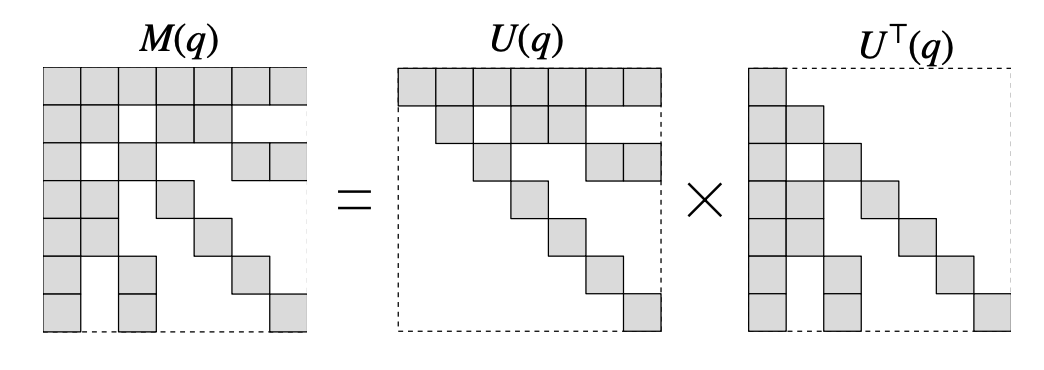
\includegraphics[width=.7\textwidth]{direct-dynamics/cholesky.png}
\end{figure}
This reduced the complexity to $O(n^2)$ when using a dense Cholesky decomposition.

\subsubsection{The maximum dissipation principle}
We showed that the contact forces $\lambda_c$ fulfill the relation:
\begin{equation*}
    G_c(q)\lambda_c + a_{c, f}(q, \dot{q}, \ddot{q}_f) = 0
\end{equation*}
From an energetic point of view, this solution minimizes:
\begin{equation*}
    \min_{\lambda_c} \frac{1}{2}\lambda_c^\tp G_c(q)\lambda_c + \lambda_c^\tp a_{c, f}(q, \dot{q}, \ddot{q}_f)
\end{equation*}
This is equivalent to the \emph{maximum dissipation principle}, which states that the contact forces are chosen to maximize the energy dissipation in the contact. This corresponds to the dual problem of the least-action principle, formally:
\begin{equation*}
    \max_{\lambda_c} -\frac{1}{2}\underbrace{
        \left(
            G_c(q)\lambda_c+2\lambda_C^\tp a_{c, f}(q, \dot{q}, \ddot{q}_f)
        \right)
    }_{a_c(q, \dot{q}, \ddot{q}_f)}
\end{equation*}
which is the dual of the least-action principle (primal):
\begin{equation*}
    \min_{\ddot{q}} \frac{1}{2}\norm{\ddot{q}-\ddot{q}_f}^2_{M(q)} \quad\text{s.t.}\quad J_c(q)\ddot{q} + \gamma_c(q, \dot{q}) = 0
\end{equation*}

\subsection{Rigid unilateral contacts}
\subsubsection{Unilateral contact as a Nonlinear Complementarity Problem}
The rigid unilateral contact model is used when the contact between the robot and the environment is rigid, and when the robot can only push the environment. This is the case, for instance, when the robot is standing on the floor. 

When dealing with unilateral contact conditions, three conditions must be satisfied:
\begin{enumerate}
    \item \textbf{Maximum dissipation} states that the contact forces should dissipate at most the kinetic energy:
    \begin{equation*}
        \min_{\lambda_c} \frac{1}{2}\lambda_c^\tp G_c(q)\lambda_c + \lambda_c^\tp a_{c, f}(q, \dot{q}, \ddot{q}_f)
    \end{equation*}
    \item \textbf{Complementary condition} (Signorini's conditions) require that the floor can \textbf{only push} (no pulling), and should emit no force when the contact is about to open:
    \begin{equation*}
        0\leq\lambda_{c,n} \perp a_{c,n}\geq 0
    \end{equation*}
    \item \textbf{Friction cone constraint} (Coulomb law) bounds the lateral forces by the normal force:
    \begin{equation*}
        \sqrt{\lambda_{c,x}^2 + \lambda_{c,y}^2} \leq \mu\lambda_{c,n}
    \end{equation*}
\end{enumerate}

\begin{figure}[H]
    \centering
    \begin{minipage}{0.4\textwidth}
        \centering
        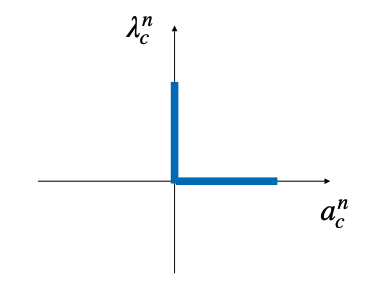
\includegraphics[width=.9\textwidth]{direct-dynamics/signorini.png}
        \caption*{Signorini's conditions}
    \end{minipage}
    \begin{minipage}{0.4\textwidth}
        \centering
        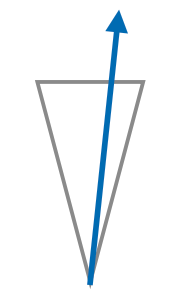
\includegraphics[width=.43\textwidth]{direct-dynamics/coulomb.png}
        \caption*{Coulomb law}
    \end{minipage}
\end{figure}

The contact problem then corresponds to a \emph{Nonlinear Complementarity Problem (NCP)}:
\begin{equation*}
    \begin{cases}
        \min_{\lambda_c} \frac{1}{2}\lambda_c^\tp G_c(q)\lambda_c + \lambda_c^\tp a_{c, f}(q, \dot{q}, \ddot{q}_f) \\
        0\leq\lambda_{c,n} \perp a_{c,n}\geq 0 \\
        \sqrt{\lambda_{c,x}^2 + \lambda_{c,y}^2} \leq \mu\lambda_{c,n}
    \end{cases}
\end{equation*}
which is non-convex, hence hard to solve. More complex solvers can be used to solve this problem in an exact way.

\subsubsection{Relaxed contact problem}
Another approach to solve the rigid unilateral contact problem is to relax the contact conditions. This is done by removing the complementarity condition, and by regularizing the forces:
\begin{equation*}
    \begin{cases}
        \min_{\lambda_c} \frac{1}{2}\lambda_c^\tp (G_c(q)\textcolor{red}{+R})\lambda_c + \lambda_c^\tp a_{c, f}(q, \dot{q}, \ddot{q}_f) \\
        \sqrt{\lambda_{c,x}^2 + \lambda_{c,y}^2} \leq \mu\lambda_{c,n}\\
        \hcancel[red]{0\leq\lambda_{c,n} \perp a_{c,n}\geq 0}
    \end{cases}
\end{equation*}
where $R$ is a regularization term. This problem becomes convex, which makes it much easier to solve. Nevertheless, the solution is not exact, which might lead to some physical inconsistencies.